\part{Entrega 2}

\section{Resultados}

\subsection{Parte 1}

Para esta sección se seleccionó un reticulado de 16 vanos para una mejor visualización de los resultados. A este, se le realizaron análisis de deformación y esfuerzos internos frente a aceleraciones aplicadas en cada dirección $x$, $y$, $z$. Posteriormente, se compararon y obtuvieron los resultados pertinentes.

\subsubsection{Aceleración en Eje X}

\begin{figure}[H]
    \centering
    \begin{minipage}{0.45\textwidth}
        \centering
        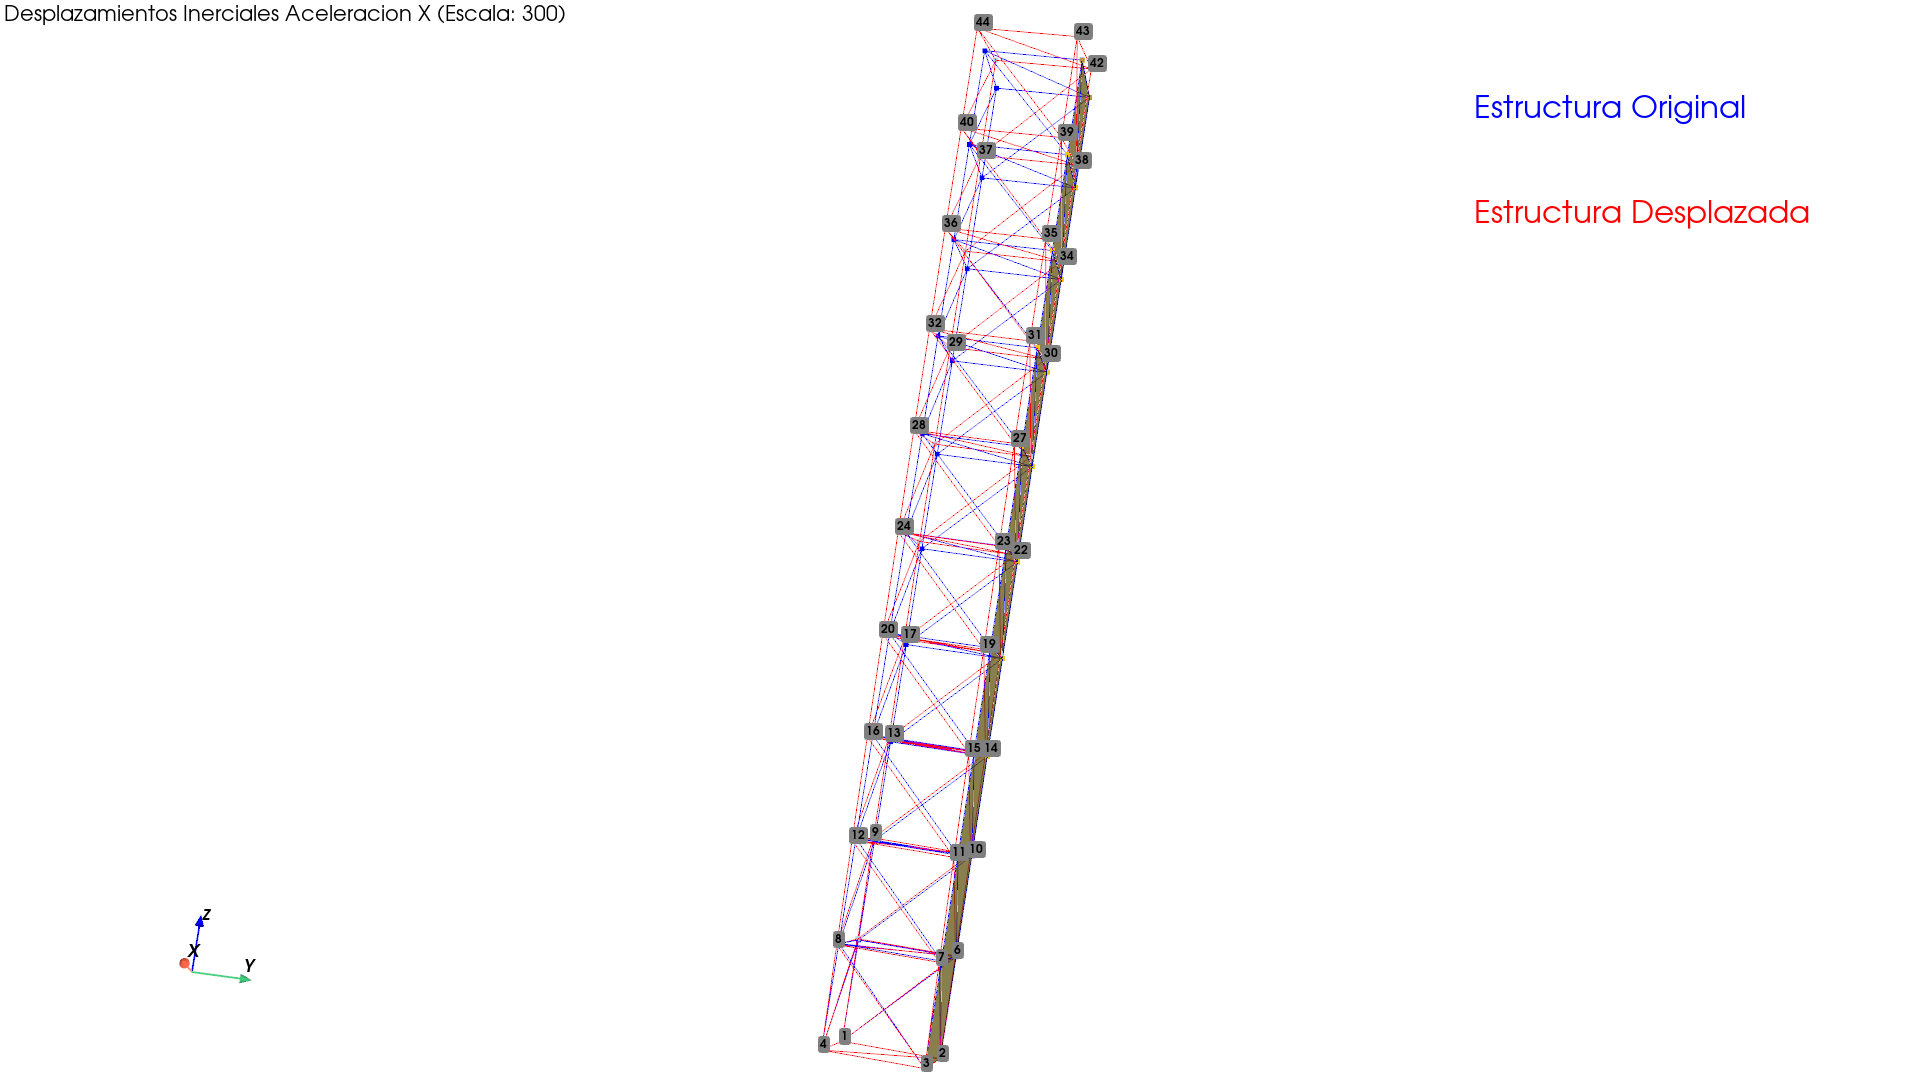
\includegraphics[width=\textwidth]{GRAFICOS/Desplazamientos Inerciales Aceleracion X False.png}
        \caption{Desplazamiento en X estructura sin diagonales cruzadas.}
        \label{fig:imagen1}
    \end{minipage}
    \hfill
    \begin{minipage}{0.45\textwidth}
        \centering
        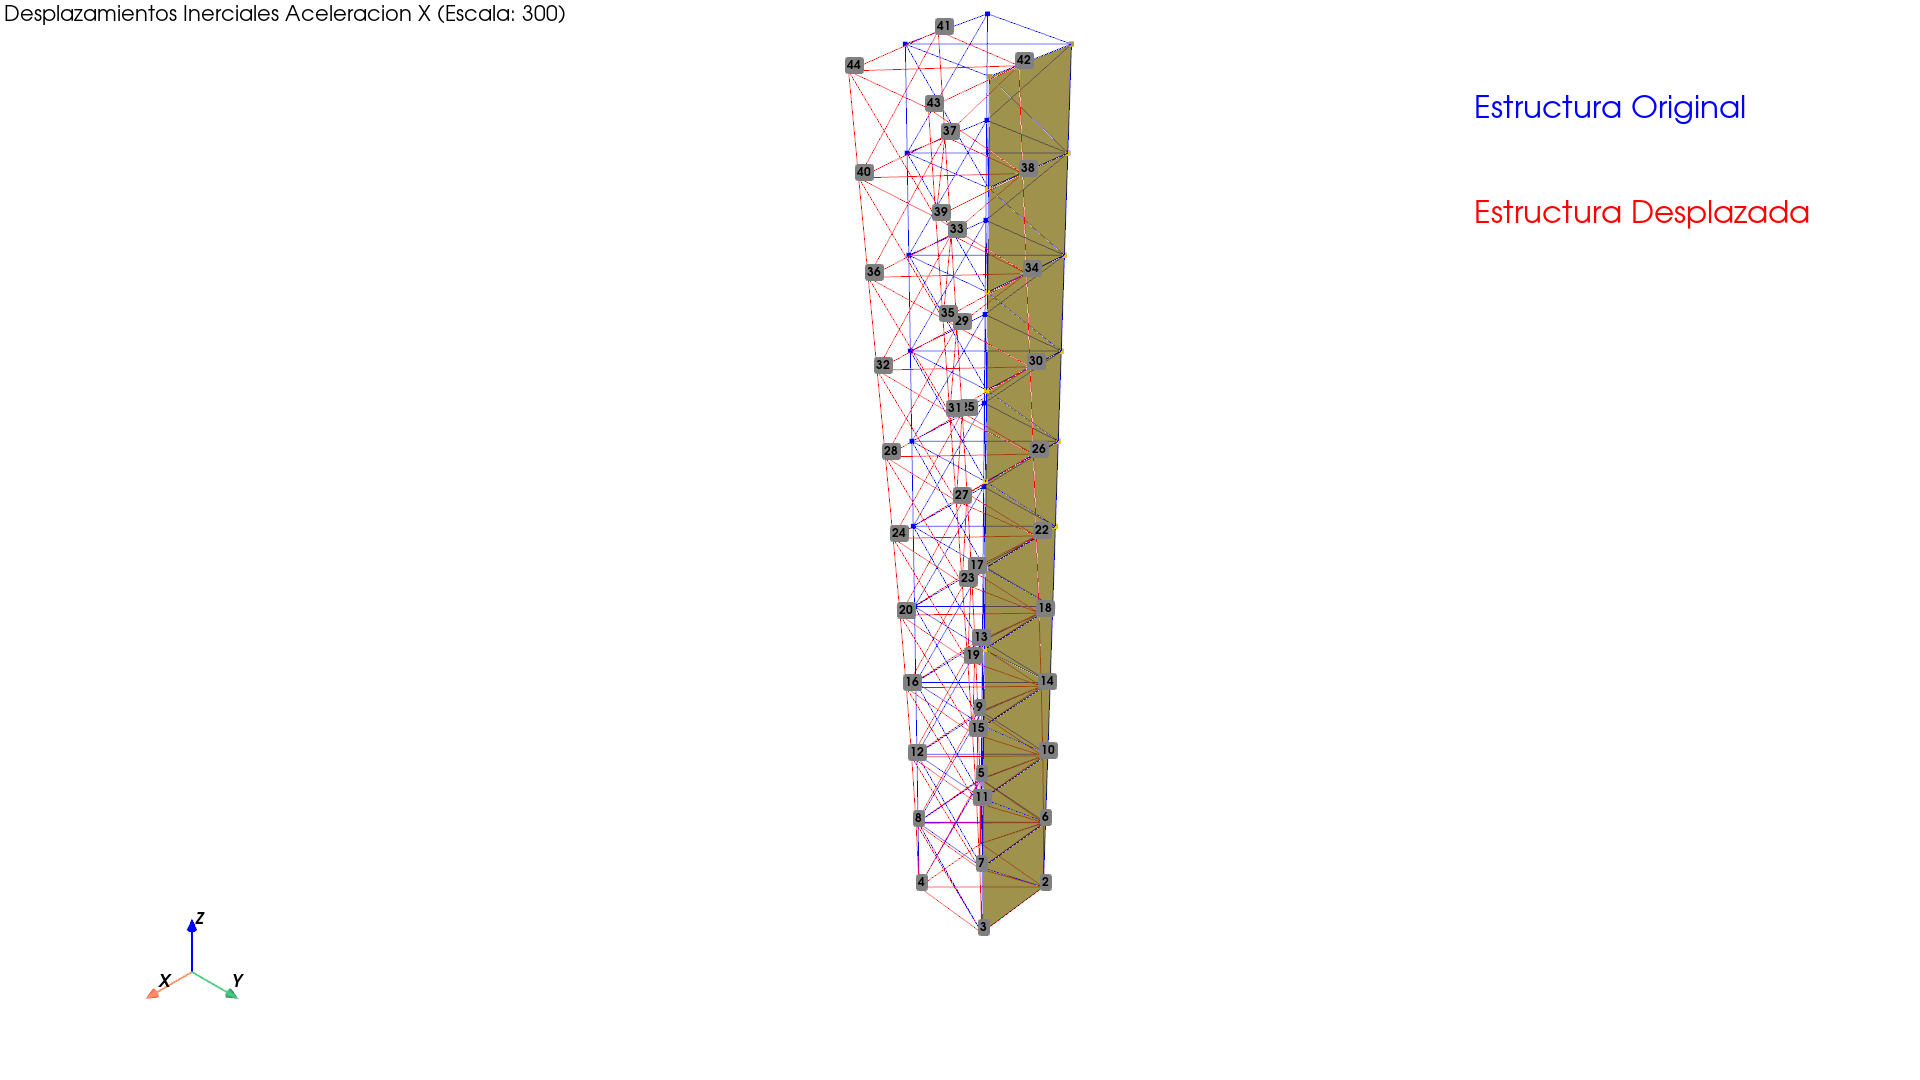
\includegraphics[width=\textwidth]{GRAFICOS/Desplazamientos Inerciales Aceleracion X True.png}
        \caption{Desplazamiento en X estructura con diagonales cruzadas.}
        \label{fig:imagen2}
    \end{minipage}
\end{figure}

\begin{figure}[H]
    \centering
    \begin{minipage}{0.45\textwidth}
        \centering
        \includegraphics[width=\textwidth]{GRAFICOS/Esfuerzos Internos Máximos en las Barras Aceleracion X False.png}
        \caption{Esfuerzos internos en estructura sin diagonales cruzadas.}
        \label{fig:imagen11}
    \end{minipage}
    \hfill
    \begin{minipage}{0.45\textwidth}
        \centering
        \includegraphics[width=\textwidth]{GRAFICOS/Esfuerzos Internos Máximos en las Barras Aceleracion X True.png}
        \caption{Esfuerzos internos en estructura con diagonales cruzadas.}
        \label{fig:imagen22}
    \end{minipage}
\end{figure}

\subsubsection{Aceleración en Eje Y}

\begin{figure}[H]
    \centering
    \begin{minipage}{0.45\textwidth}
        \centering
        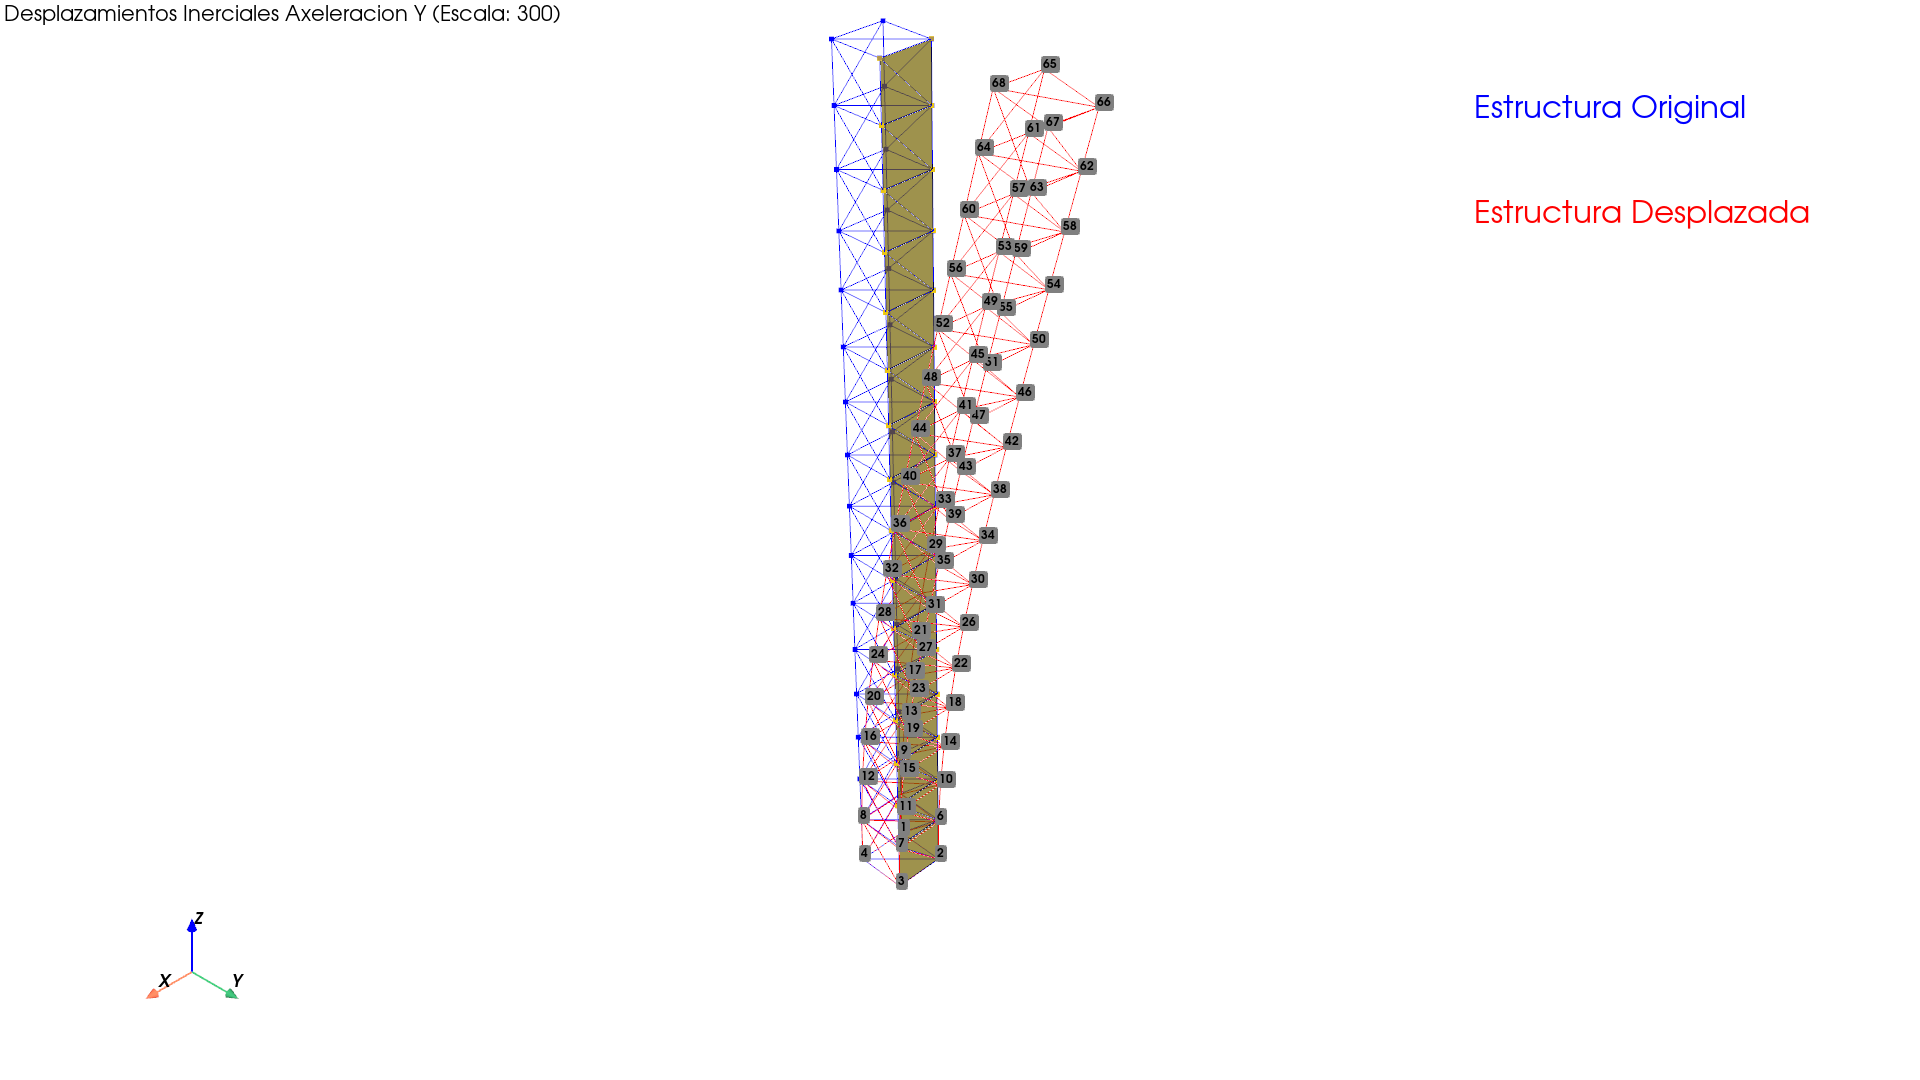
\includegraphics[width=\textwidth]{GRAFICOS/Desplazamientos Inerciales Axeleracion Y False.png}
        \caption{Desplazamiento en Y estructura sin diagonales cruzadas.}
        \label{fig:imagen3}
    \end{minipage}
    \hfill
    \begin{minipage}{0.45\textwidth}
        \centering
        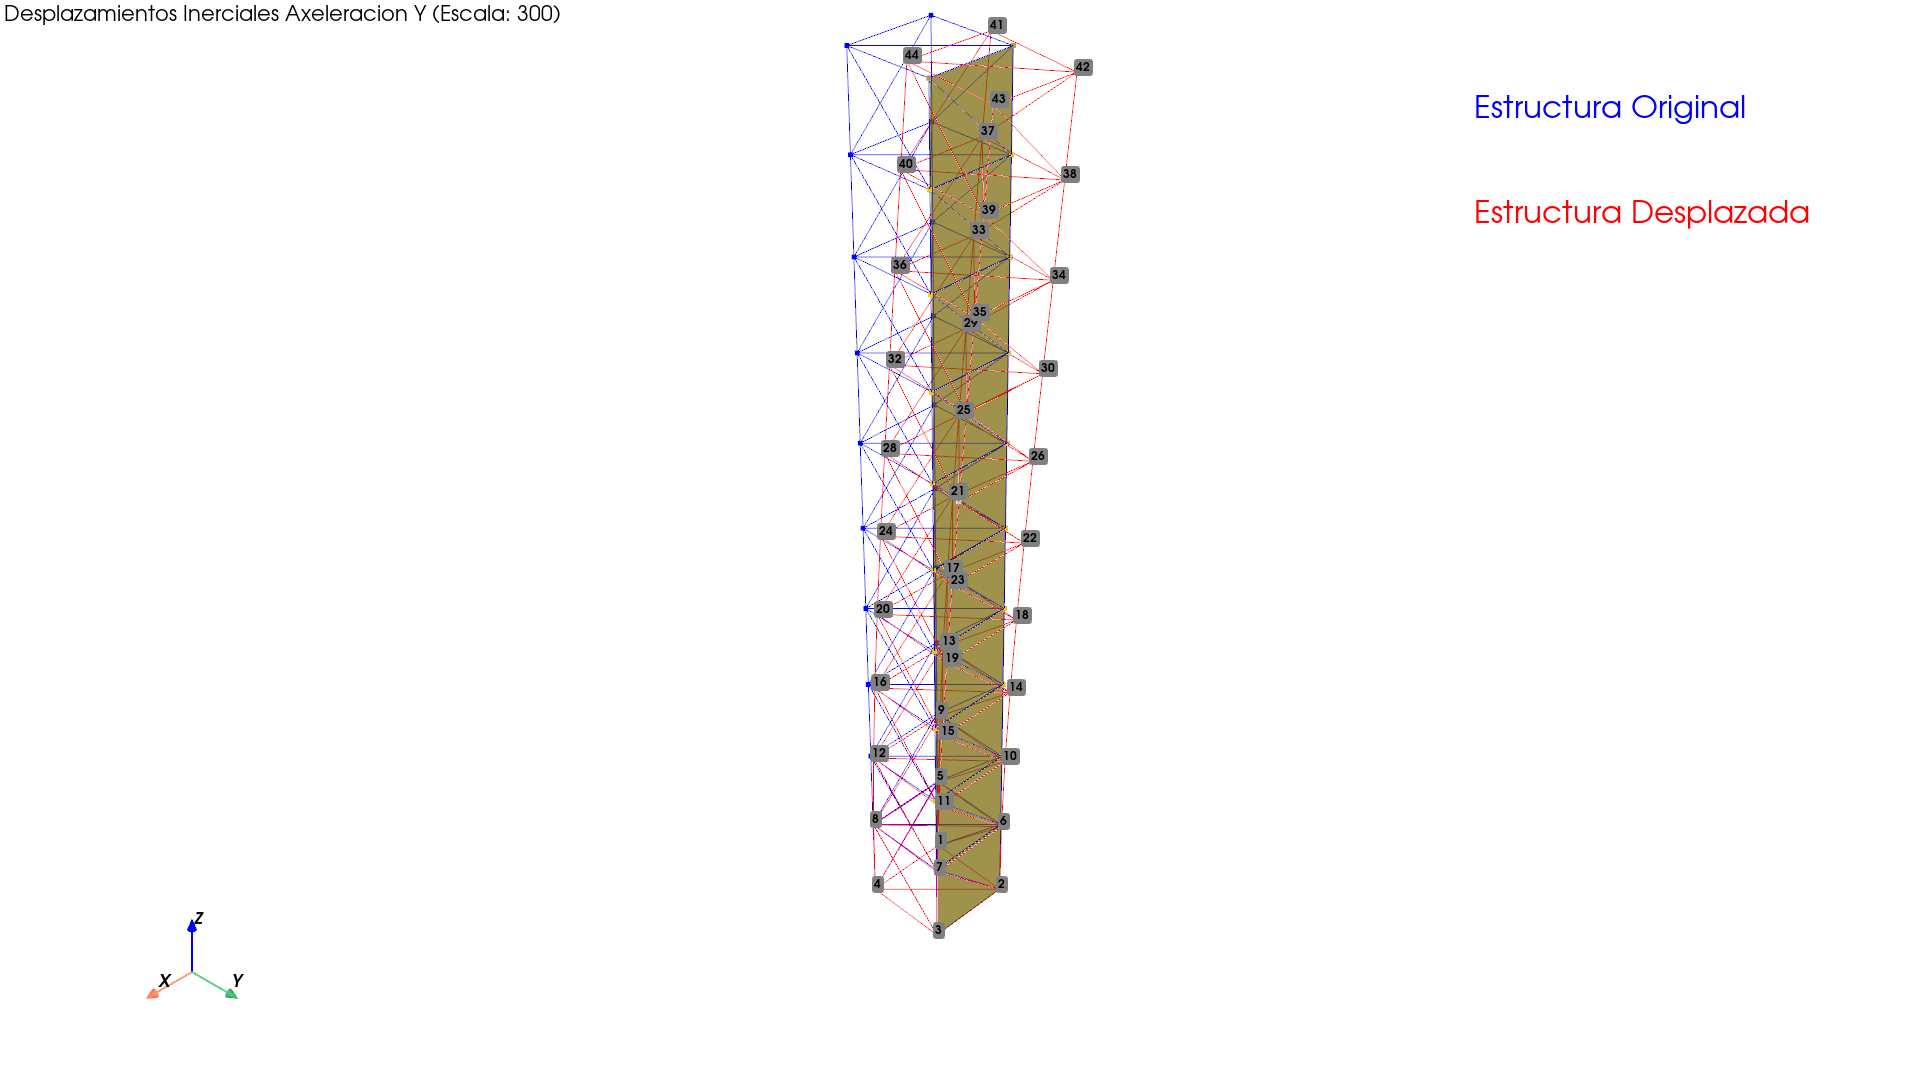
\includegraphics[width=\textwidth]{GRAFICOS/Desplazamientos Inerciales Axeleracion Y True.png}
        \caption{Desplazamiento en Y estructura con diagonales cruzadas.}
        \label{fig:imagen4}
    \end{minipage}
\end{figure}

\begin{figure}[H]
    \centering
    \begin{minipage}{0.45\textwidth}
        \centering
        \includegraphics[width=\textwidth]{GRAFICOS/Esfuerzos Internos Máximos en las Barras Axeleracion Y False.png}
        \caption{Esfuerzos internos en estructura sin diagonales cruzadas.}
        \label{fig:imagen33}
    \end{minipage}
    \hfill
    \begin{minipage}{0.45\textwidth}
        \centering
        \includegraphics[width=\textwidth]{GRAFICOS/Esfuerzos Internos Máximos en las Barras Axeleracion Y True.png}
        \caption{Esfuerzos internos en estructura con diagonales cruzadas.}
        \label{fig:imagen44}
    \end{minipage}
\end{figure}

\subsubsection{Aceleración en Eje Z}

\begin{figure}[H]
    \centering
    \begin{minipage}{0.45\textwidth}
        \centering
        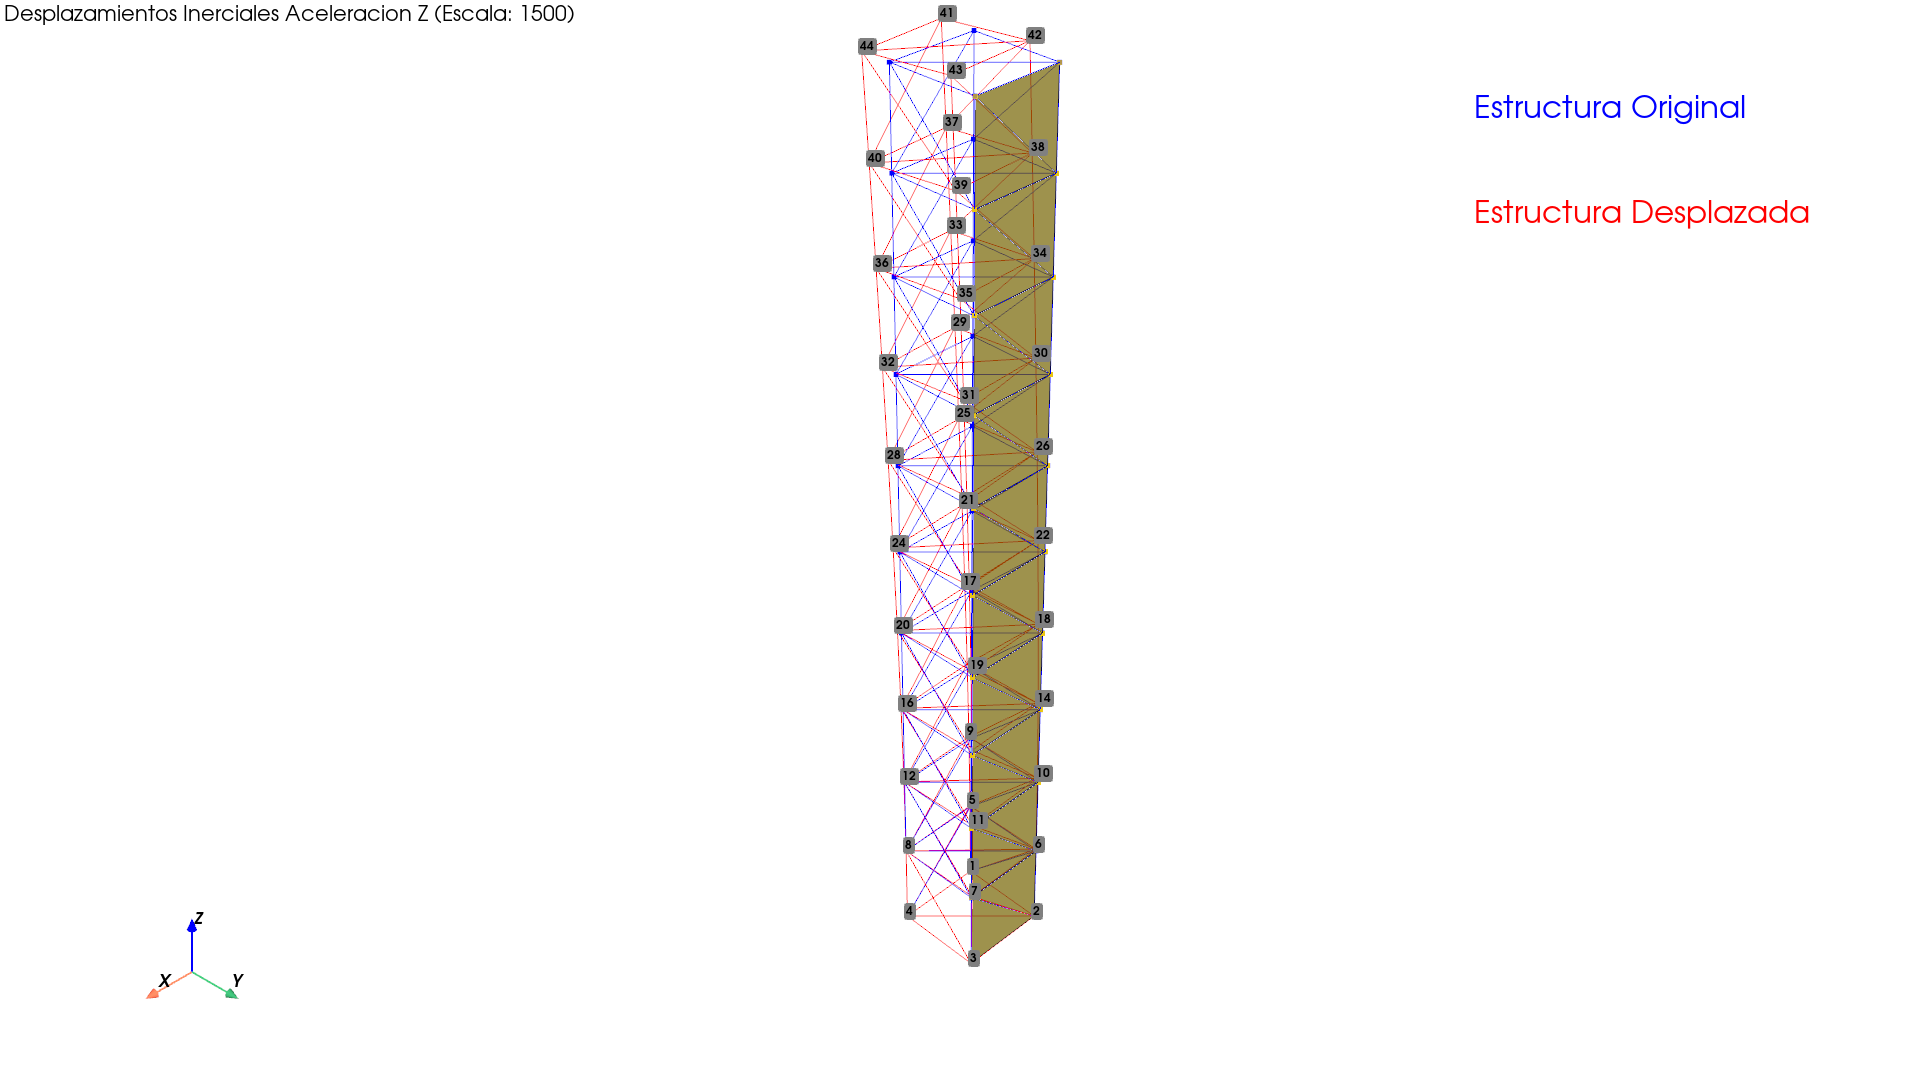
\includegraphics[width=\textwidth]{GRAFICOS/Desplazamientos Inerciales Aceleracion Z False.png}
        \caption{Desplazamiento en Z estructura sin diagonales cruzadas.}
        \label{fig:imagen5}
    \end{minipage}
    \hfill
    \begin{minipage}{0.45\textwidth}
        \centering
        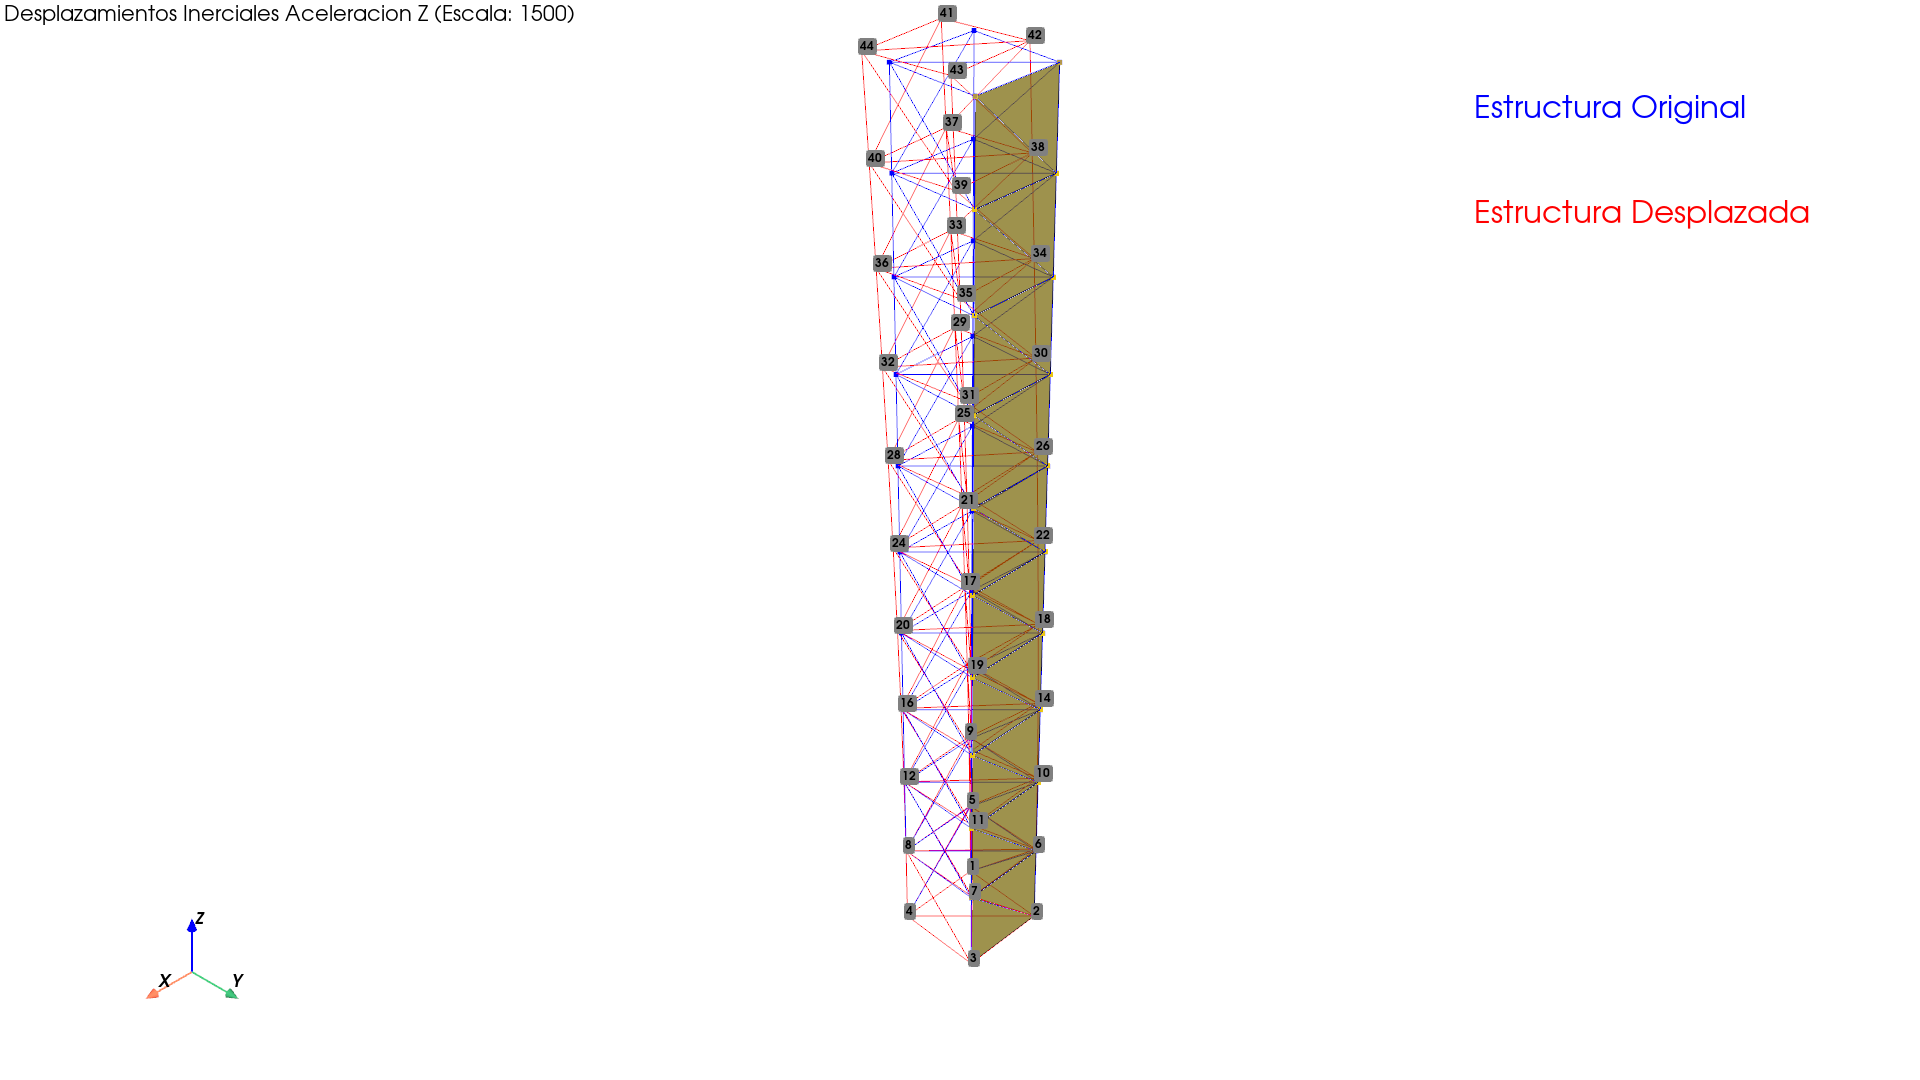
\includegraphics[width=\textwidth]{GRAFICOS/Desplazamientos Inerciales Aceleracion Z True.png}
        \caption{Desplazamiento en Z estructura con diagonales cruzadas.}
        \label{fig:imagen6}
    \end{minipage}
\end{figure}

\begin{figure}[H]
    \centering
    \begin{minipage}{0.45\textwidth}
        \centering
        \includegraphics[width=\textwidth]{GRAFICOS/Esfuerzos Internos Máximos en las Barras Aceleracion Z False.png}
        \caption{Esfuerzos internos en estructura sin diagonales cruzadas.}
        \label{fig:imagen55}
    \end{minipage}
    \hfill
    \begin{minipage}{0.45\textwidth}
        \centering
        \includegraphics[width=\textwidth]{GRAFICOS/Esfuerzos Internos Máximos en las Barras Aceleracion Z True.png}
        \caption{Esfuerzos internos en estructura con diagonales cruzadas.}
        \label{fig:imagen66}
    \end{minipage}
\end{figure}

\subsubsection{Aumento de temperatura en 100°C en nodos conectados al panel}

\begin{figure}[H]
    \centering
    \begin{minipage}{0.45\textwidth}
        \centering
        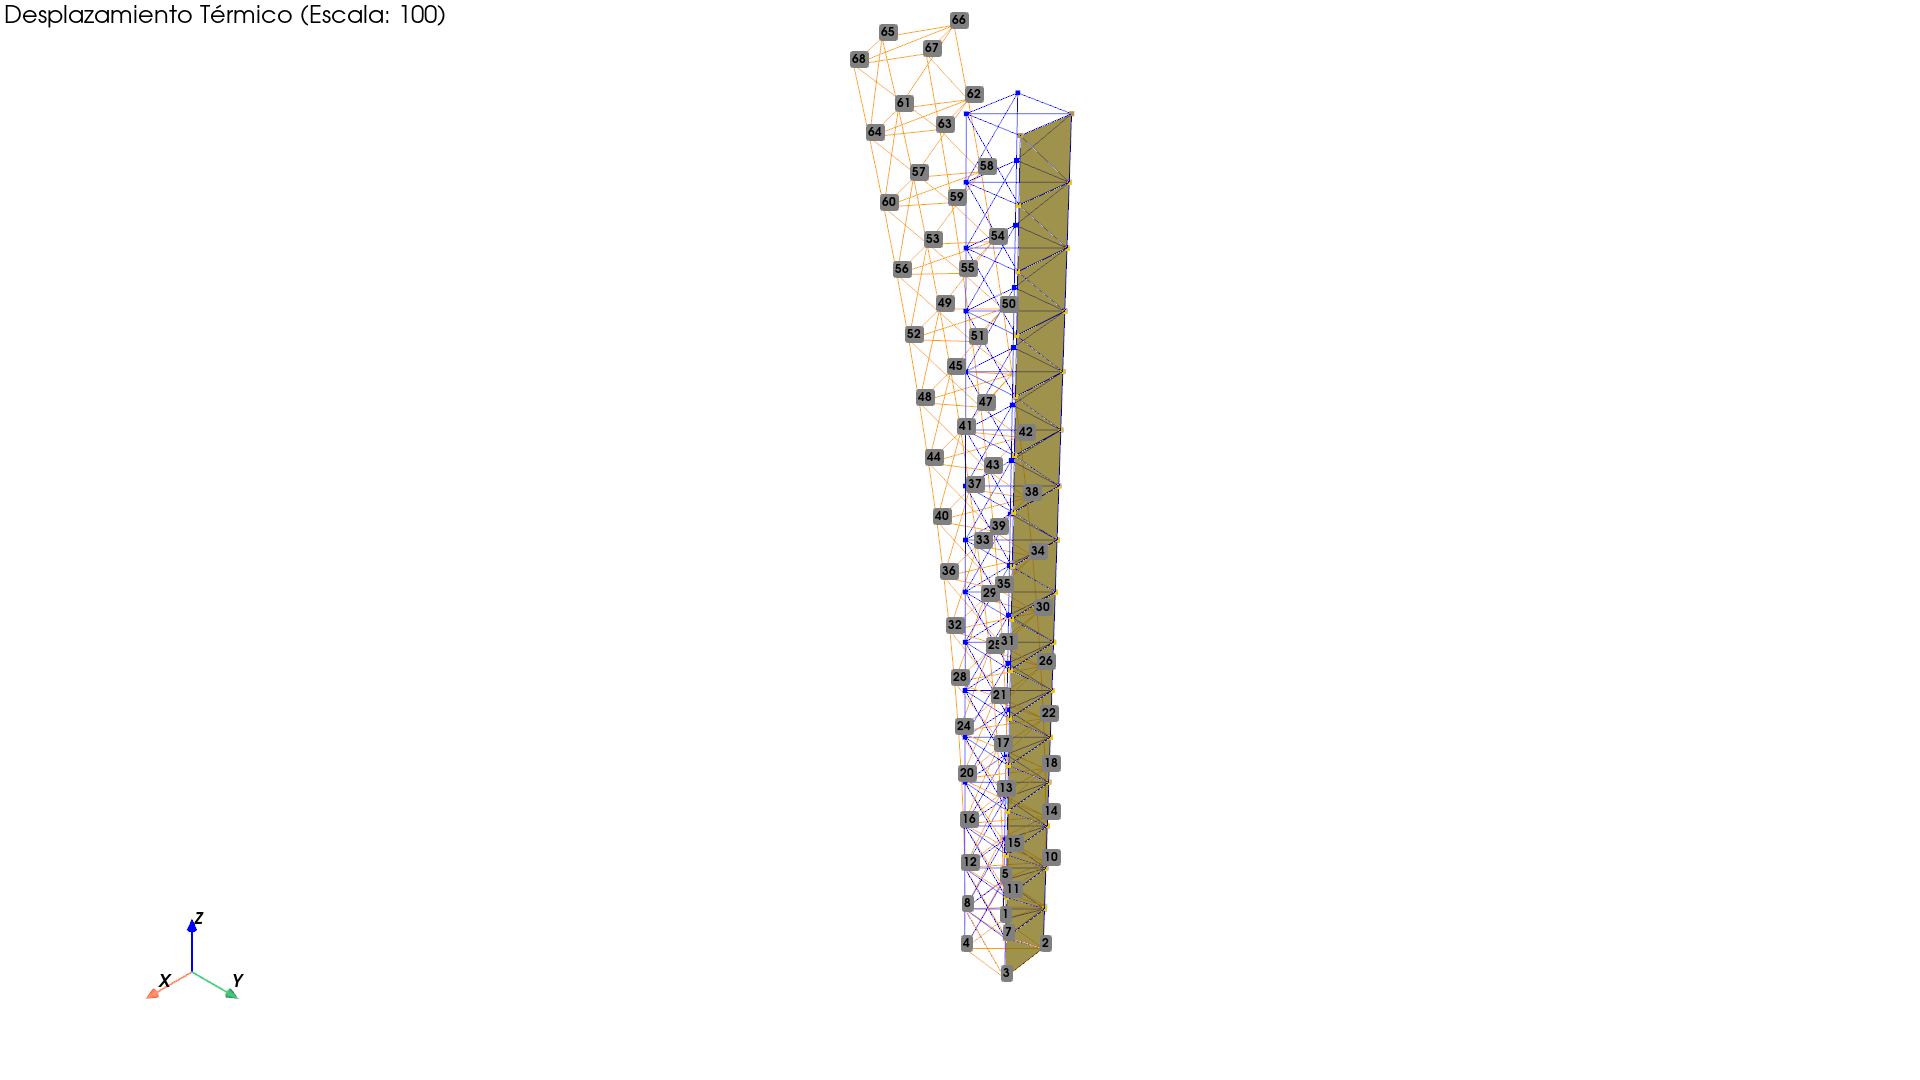
\includegraphics[width=\textwidth]{GRAFICOS/Desplazamientos Termicos False.png}
        \caption{Desplazamiento $\Delta T$ en estructura sin diagonales cruzadas.}
        \label{fig:imagen7}
    \end{minipage}
    \hfill
    \begin{minipage}{0.45\textwidth}
        \centering
        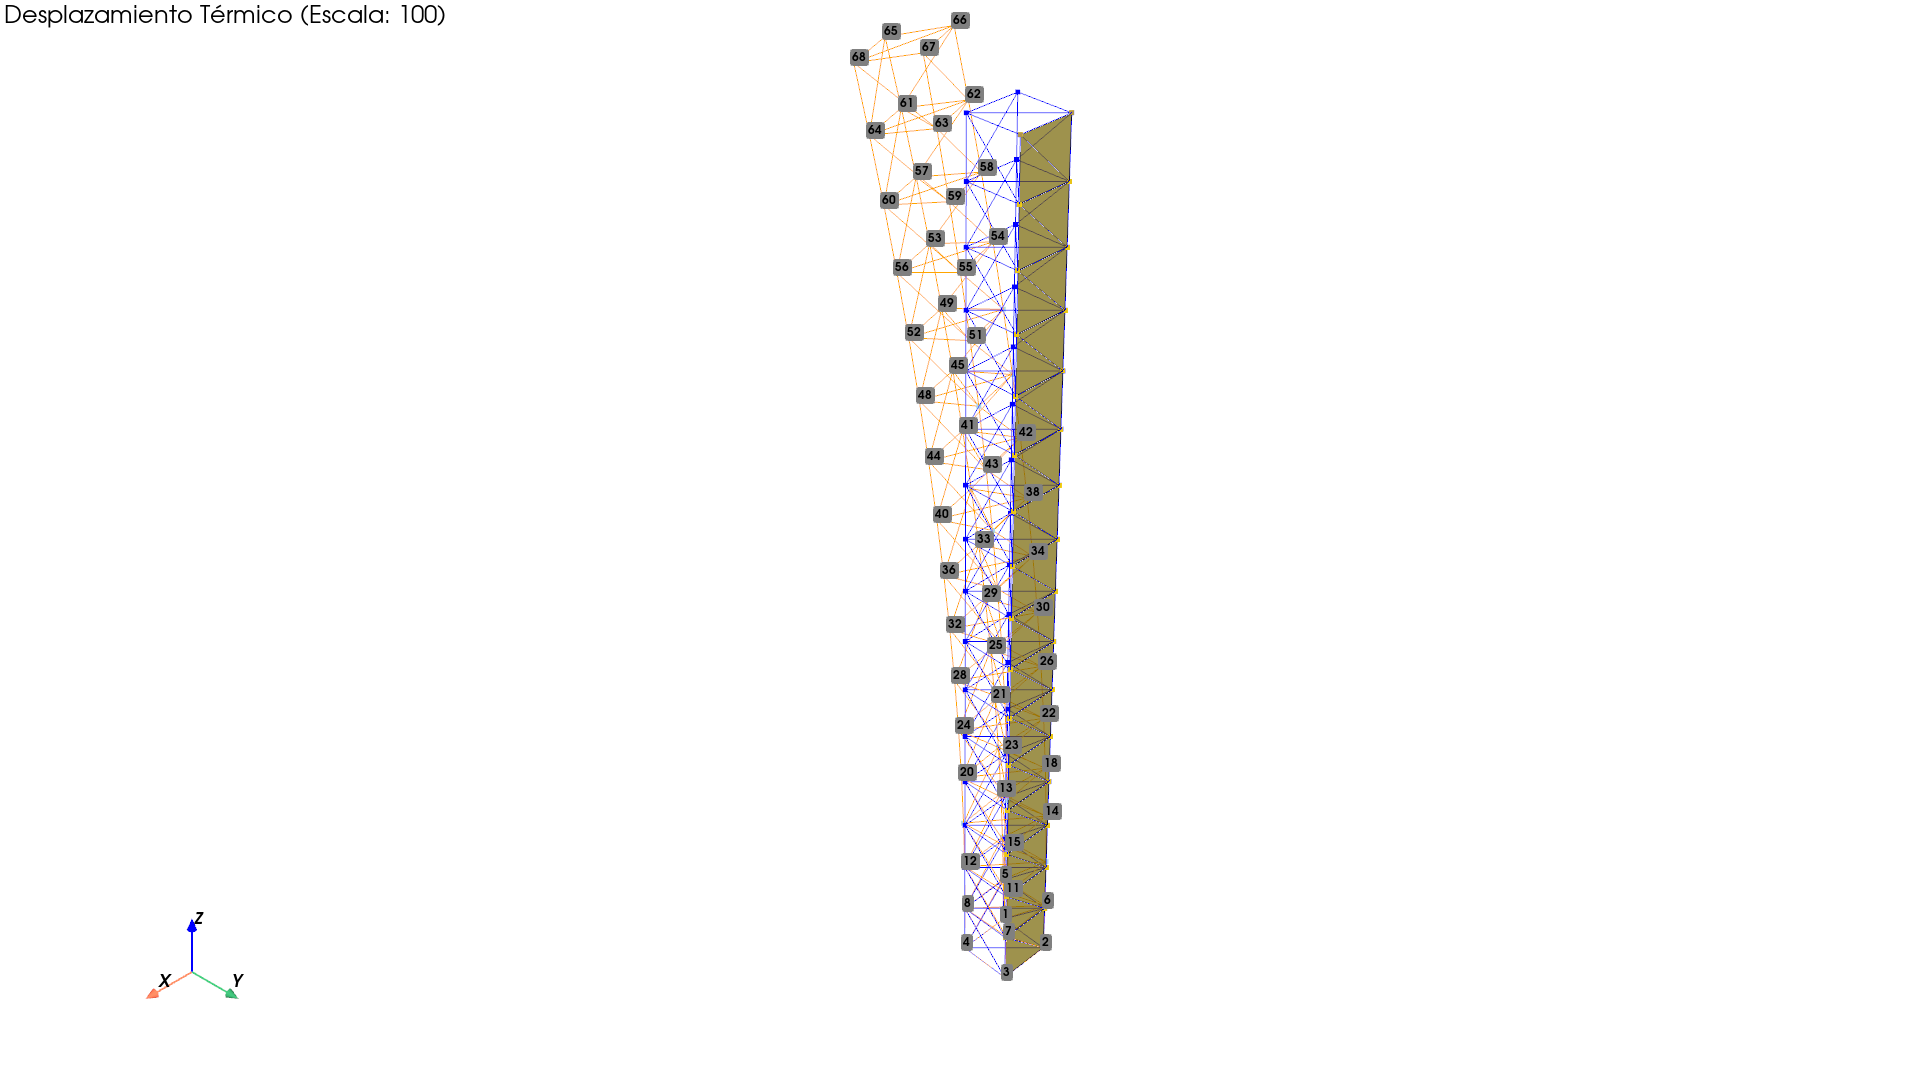
\includegraphics[width=\textwidth]{GRAFICOS/Desplazamientos Termicos True.png}
        \caption{Desplazamiento $\Delta T$ en estructura con diagonales cruzadas.}
        \label{fig:imagen8}
    \end{minipage}
\end{figure}

\begin{figure}[H]
    \centering
    \begin{minipage}{0.45\textwidth}
        \centering
        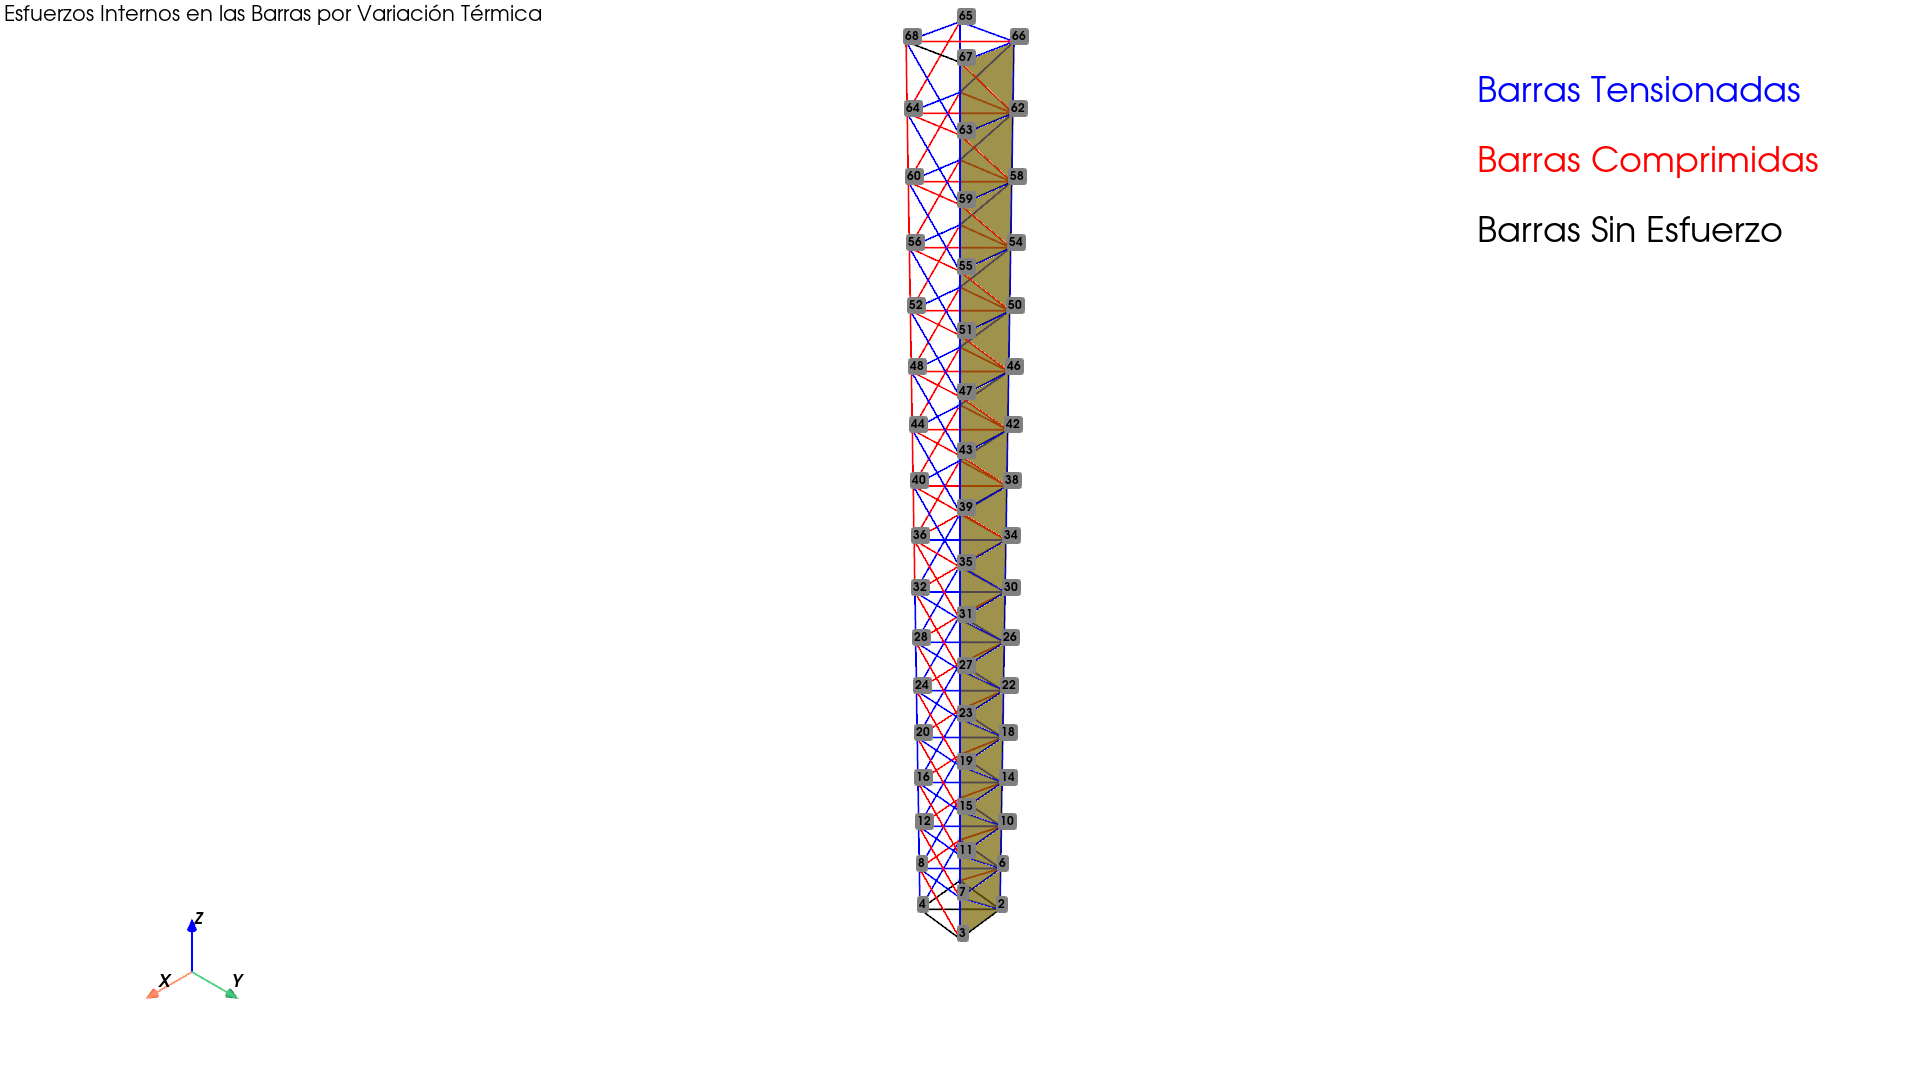
\includegraphics[width=\textwidth]{GRAFICOS/Esfuerzos Internos en las Barras por Variación Térmica False.png}
        \caption{Esfuerzos internos por $\Delta T$ en estructura sin diagonales cruzadas.}
        \label{fig:imagen77}
    \end{minipage}
    \hfill
    \begin{minipage}{0.45\textwidth}
        \centering
        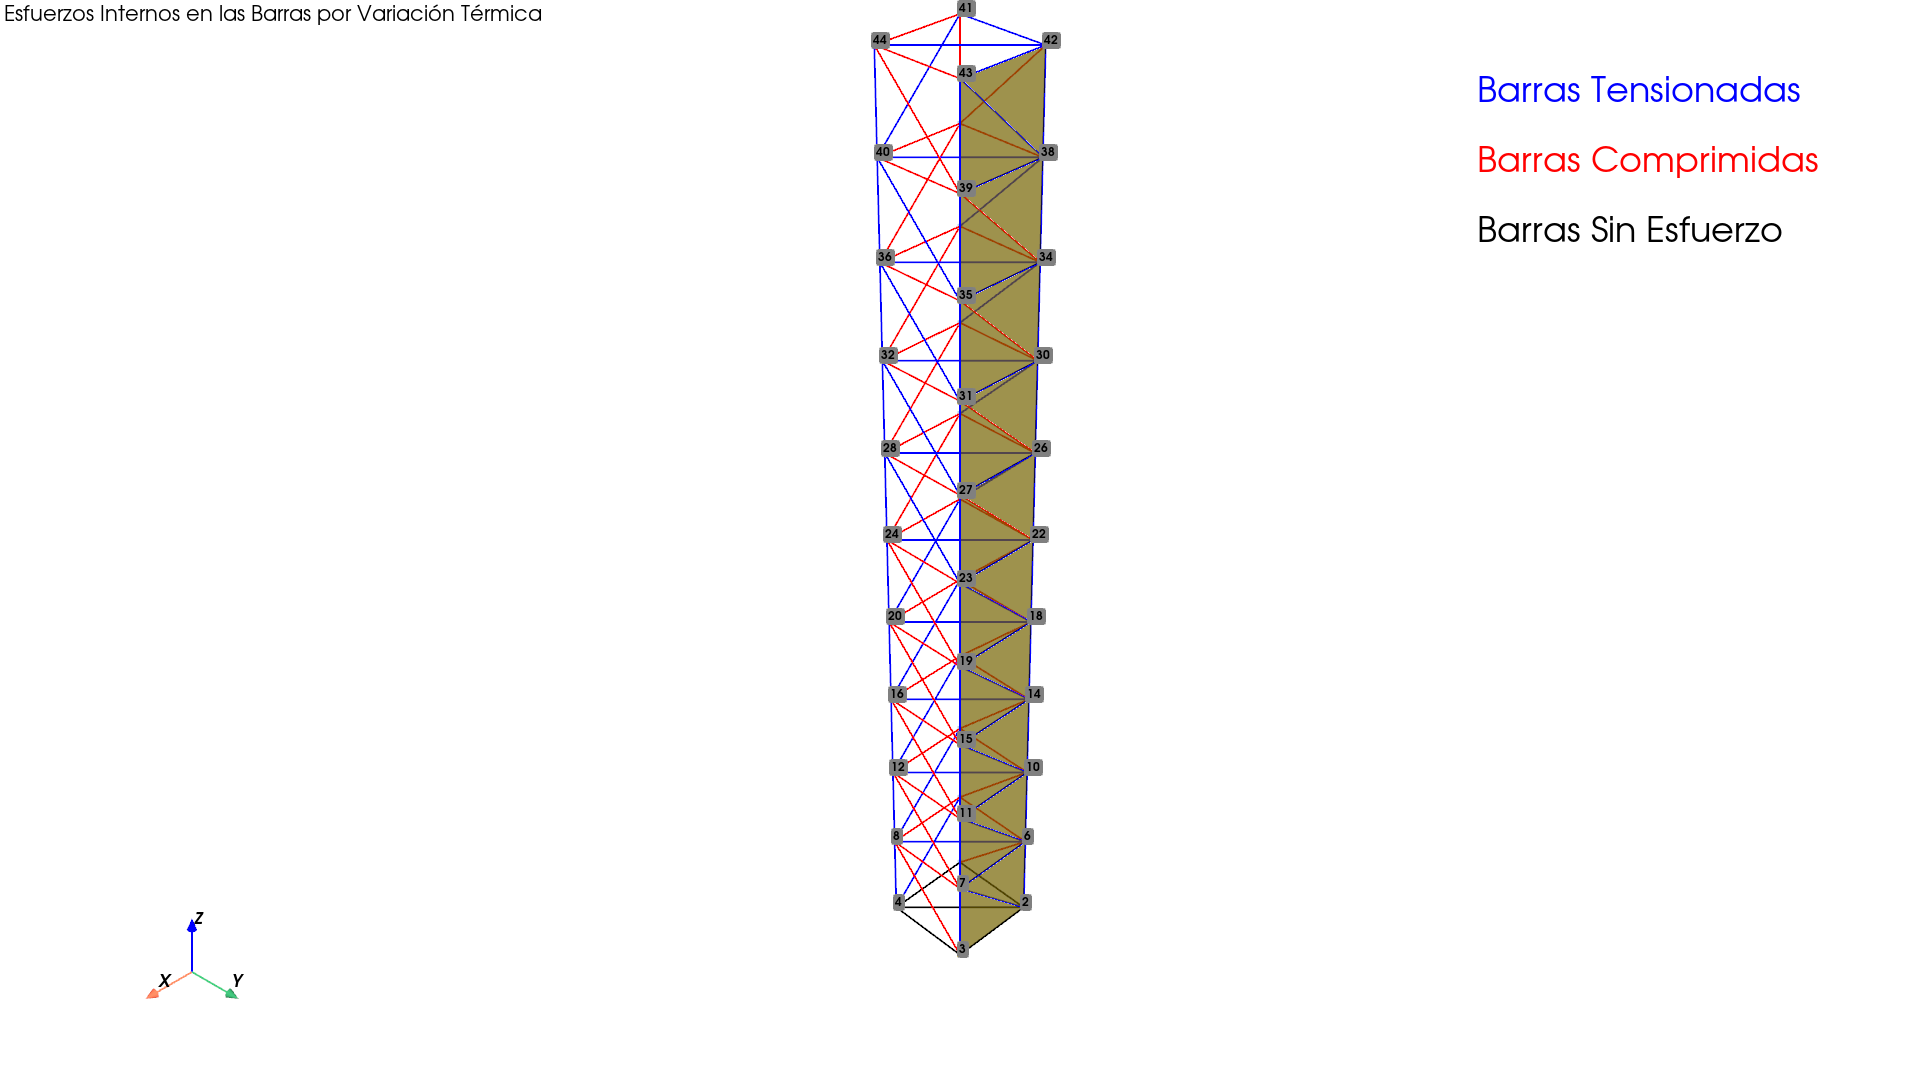
\includegraphics[width=\textwidth]{GRAFICOS/Esfuerzos Internos en las Barras por Variación Térmica True.png}
        \caption{Esfuerzos internos por $\Delta T$ en estructura con diagonales cruzadas.}
        \label{fig:imagen88}
    \end{minipage}
\end{figure}










